\documentclass[12pt,a4paper]{article}
\usepackage[parfill]{parskip}
\usepackage{fullpage}
\usepackage{enumitem}
\usepackage{hyperref}
\usepackage{graphicx}
\usepackage{subfig}
\usepackage{amsmath}
\begin{document}

\vfil

\begin{center}
	{\Large Mobile Robot Systems} \\
	\vspace{0.4in}
	{\huge \bf Assignment 1 } \\
	\vspace{0.4in}
	{\large Anik Roy} \\
	\vspace{0.1in}
	{\large \today} \\
\end{center}
\vspace{0.4in}

% Main document

\section*{1.1 Dynamical Systems and Motion Control}
\subsection*{Exercise 1}
\begin{enumerate}[label=(\alph*)]
		\item $\dot{x} = u\cdot cos(\theta)$\\
	      $\dot{y} = u\cdot sin(\theta)$\\
	      $\omega = cos(t)$
        \item The solution uses Euler's method for approximating the solution to a differential equation. The starting point is decided, then the gradient is computed. A small step (of size dt) is taken along the tangent line computed. The new point is taken as the new starting point, and the procedure continues funcding consecutive points, approximating the curve (which is the solution to the differential equation). In my solution, the poses are the points, where the next pose is calculated by adding the previous pose to the increase in each component. This increase is calculated from the differential equations (which give us the rate of increase of $x$, $y$ and $\theta$). Multiplying the rate of increase by the change in time (dt), gives the amount by which to increase each component to get the next position. This only approximates the position since there will be an error since the gradient will change within the dt.
		\item The plot here shows the output of Euler's method with varying step sizes. Smaller step sizes gives a smoother looking curve, since the curve is made up of smaller individual segments. The smaller step size also means that it is closer to the real curve since the tangent lines that euler produces won't go as far away from the real curve.  A smaller step size takes longer to compute, but will produce a solution which is a closer approximation to the real (exact) solution. A larger step size will be quicker to run, but a worse approximation.
	      \begin{figure}[h!]
	      	\centering
	      	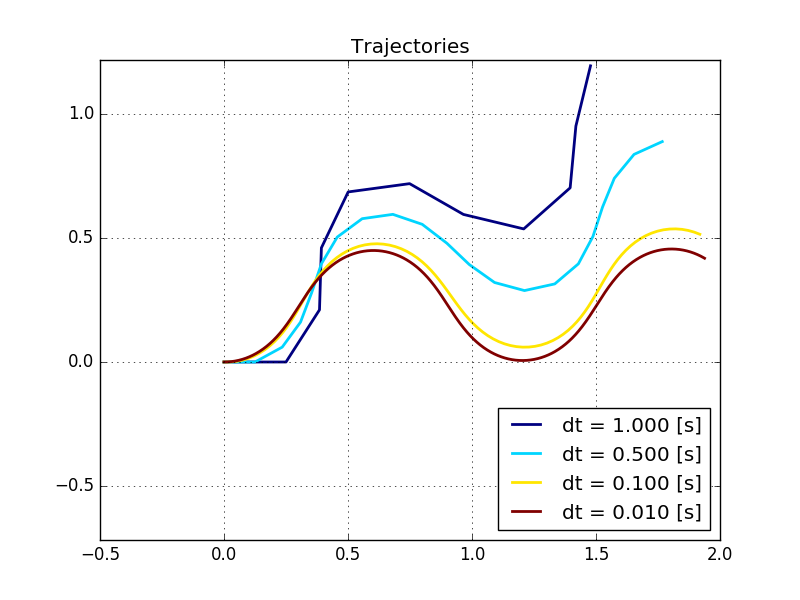
\includegraphics[width=\textwidth]{fig/1c.png}
	      	\caption{Euler's method}
	      	\label{fig:euler}
	      \end{figure}
	\item RK4 is another method for approximating a solution to differential equations. Instead of just using one gradient to calculate a single tangent line, it calculates 4 gradients and combines them to produce subsequent points that are closer to the real curve. In my solution, I calculate the four components that make up the change in theta (one at the start, two halfway across the step size, one at the end of the step) and combine them, weighting them accordingly. I then use these components in calculating the change in $x$ an $y$. Since $\dot{x}$ and $\dot{y}$ are only functions of theta, we need to use these components as arguments to the function.\\
	The equations I used:\\ \\
		  $ \theta_{n+1} = \theta_n + {1\over{6}} (k_1 + 2k_2 + 2k_3 + k_4) $\\
		$k_1 = h\cdot cos(t)$\\
		$k_2 = h\cdot cos(t+h/2)$\\
		$k_3 = h\cdot cos(t+h/2)$\\
		$k_4 = h\cdot cos(t+h)$\\

		$ x_{n+1} = x_n + {1\over{6}} (k_1x + 2k_2x + 2k_3x + k_4x) $\\
		$k_1x = h \cdot u \cdot cos(\theta)$\\
		$k_2x = h \cdot u \cdot cos(\theta+k_1/2)$\\
		$k_3x = h \cdot u \cdot cos(\theta+k_2/2)$\\
		$k_4x = h \cdot u \cdot cos(\theta+k_3)$\\
		
		$ y_{n+1} = y_n + {1\over{6}} (k_1y + 2k_2y + 2k_3y + k_4y) $\\
		$k_1y = h \cdot u \cdot cos(\theta)$\\
		$k_2y = h \cdot u \cdot cos(\theta+k_1/2)$\\
		$k_3y = h \cdot u \cdot cos(\theta+k_2/2)$\\
		$k_4y = h \cdot u \cdot cos(\theta+k_3)$\\
		
	\item Figure \ref{fig:rk4} shows the plot using rk4 instead of Euler. There are several differences between RK4 and Euler. The main one is that Euler is a first order method, and RK4 is a fourth order method, so the error in euler's method decreases on the order of $O(h)$, whereas RK4 is $O(h^4)$, where h is the step size. As the step size gets smaller, the error (difference to exact solution) using RK4 will decrease faster than when using Euler. Euler's method only looks at the single gradient taken at each point to construct a line parallel to the tangent at the curve, whereas RK4 looks at 4 gradients within the step size, and weights them to compute the next point. Taking into account this extra information allows it to converge to the solution quicker. Euler's method can produce acceptable results when the gradient of the curve does not change much, since the error will be smaller. Euler's method is also easier to code and will be quicker to run since it will have to do less calculations. However, it will need a much smaller step size than rk4 so it may not end up being as efficient. Euler's method can also perform better when there are discontinuities, if the step size happens to line up with those discontinuities although this is unlikely and would require a lot of tuning.
	      \begin{figure}[h!]
	      	\centering
	      	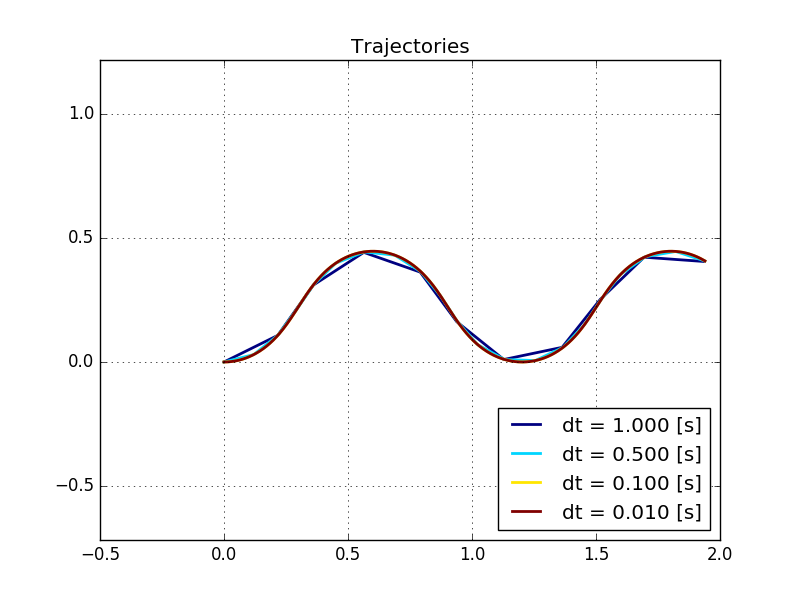
\includegraphics[width=\textwidth]{fig/1e.png}
	      	\caption{RK4}
	      	\label{fig:rk4}
	      \end{figure}
	\item Changing $\omega$ from $cos(t)$ to $cos(\lfloor t \rfloor)$ simulates a 1Hz perception-action loop, where every second the robot will change its action. Using the euler method now produces similar plots regardless of step size. This is because the error between the approximation and the exact solution will be relatively low, since $\omega$ will not change for each timestep due to the floor function. For example, when dt is 1s, the step size is the same as how often $t$ changes. This means the error will be very small, since there is no change in $\omega$. So the smaller step sizes will make little difference in producing a better approximation with euler's method. However, with RK4, since it takes into account points from the beginning, middle and end of the step size, the floor function and so ($cos(\lfloor t \rfloor)$) will not be approximated well due to the discontinuities. This is especially worse if the steps span the discontinuities. This is why we can see that for RK4, a larger step size produces a lot of error compared to Euler. For both, a small step size will produce a good result, but the more naive method works well here.
		\begin{figure}[h!]
		\centering
		\subfloat[Euler]{{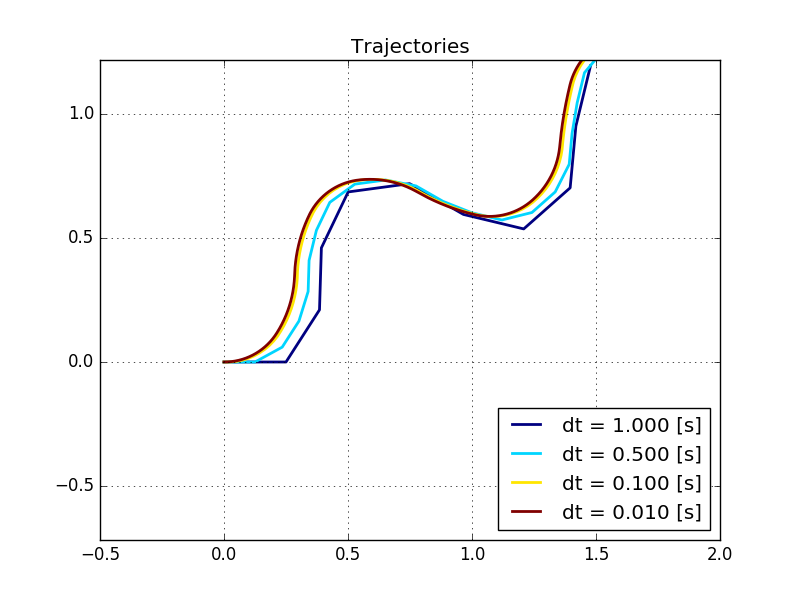
\includegraphics[width=7cm]{fig/1f-euler.png}}}%
		\qquad
		\subfloat[RK4]{{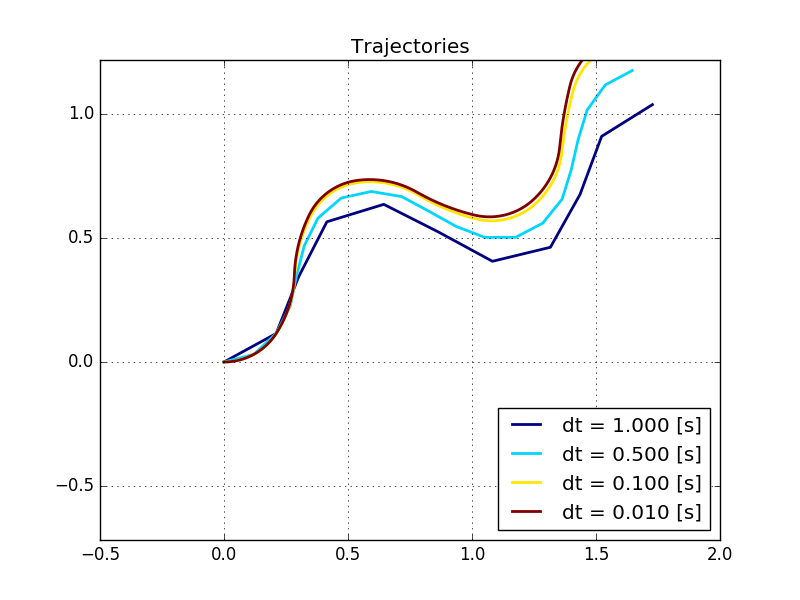
\includegraphics[width=7cm]{fig/1f-rk4-2.png}}}%
		\caption{Plots using $\omega=cos(\lfloor t \rfloor)$}%
		\label{fig:floor}%
		\end{figure}
	\item Using a fixed time step will not always be optimal, since the functions may not change much during a large part of the time step, but then change a lot in another part of the time step. In the case of the floor function, the time step needs to be large between the discontinuities, and small around the discontinuities to take into account the large jump in a very small time. I've implemented an adaptive method for Euler, with the results shown in figure \ref{fig:bonus} for different starting step sizes:
	\begin{figure}[h!]
		\centering
		\subfloat[Euler]{{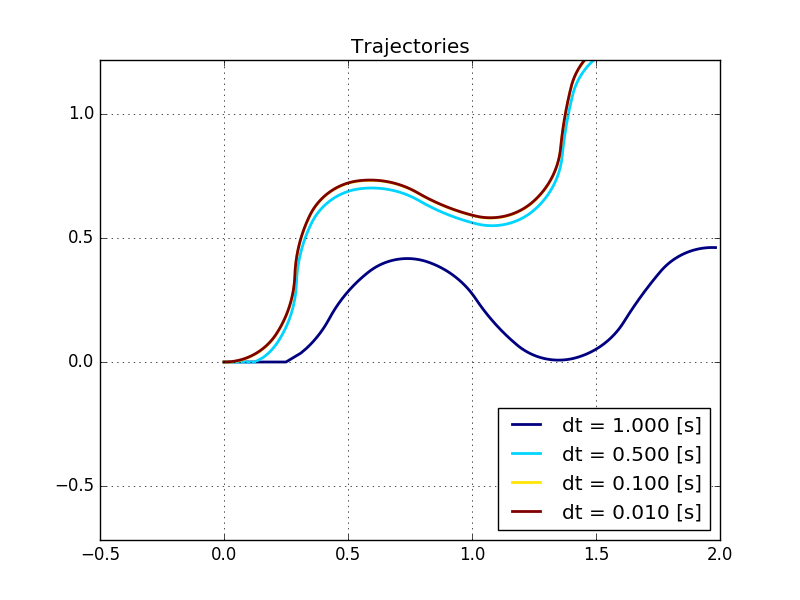
\includegraphics[width=7cm]{fig/1g-euler.png}}}%
		\qquad
		\subfloat[RK4]{{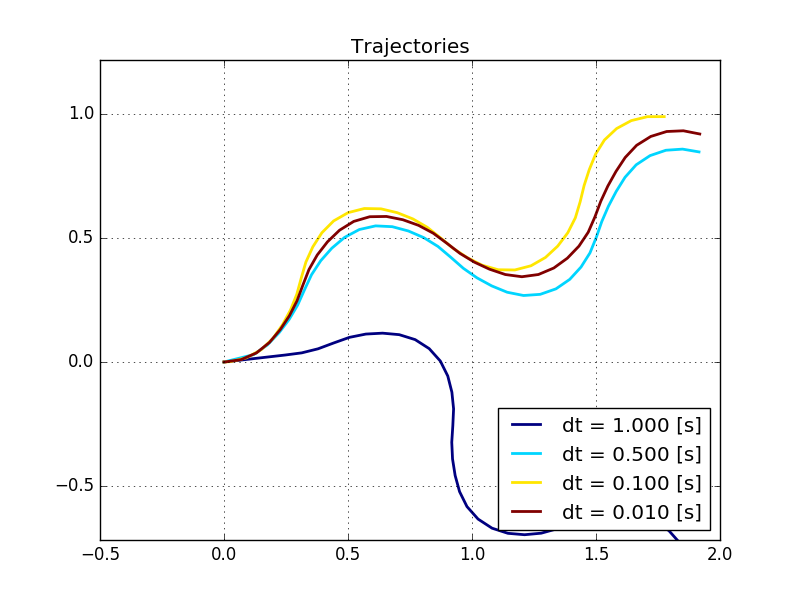
\includegraphics[width=7cm]{fig/1g-rk4.png}
		}}%
		\caption{Euler's method with an adaptive step size, dt here is starting step size}		
		\label{fig:bonus}%
		\end{figure}

	For each point, I do a standard iteration of euler with the given step size, as well as two iterations with half the step size. I then compare the results, and find the sum of the component differences between the two as a proxy for the error. Using this error, I find the next step size by choosing a larger step size for lower errors, and a smaller step size for larger errors, according to the formula below\footnote{tuned from the example at https://en.wikipedia.org/wiki/Adaptive\_stepsize}. I also use the same method for rk4:

	$$dt=0.9 \cdot min(max(1/error,0.3),2)$$

	The min and max make sure the dt stays within some bounds.

\end{enumerate}
\subsection*{Exercise 2}
\begin{enumerate}[label=(\alph*)]
        \item The plot of my braitenburg controller is shown in Figure \ref{fig:braitenburg}. The velocity is a function of the reciprocal of the sensors. Using the reciprocal allows the case where the obstacle is further than 3.5 (infinity) becomes 0. For the rotational velocity, this is also function of the reciprocal of the sensors - when the robot is close to an obstacle, it should rotate faster to get away. Since we want to move away from obstacles (the 'coward' example from lecture 4), the rotational velocity will increase (counter-clockwise) if the robot senses it is closer to objects on the right, and vice versa for objects on the left. Both velocities are made up of weighted components of the indivdual sensor values. I estimated and tuned these weights by trial and error. The result is a matrix multiplication of the weights by the sensor values to produce a column vector of $u$ and $\omega$. The $m_i$ in the equation below are the sensor measurements, and the $w_ij$ are the weights.

		\begin{equation*}
			\begin{pmatrix}
				u\\
				\omega
			\end{pmatrix}
			=
			\begin{pmatrix}
				w_{11} & w_{12} & w_{13} & w_{14} & w_{15}\\
				w_{21} & w_{22} & w_{23} & w_{24} & w_{25}
			\end{pmatrix}
			\cdot
			\begin{pmatrix}
				\frac{1}{m_1}\\
				\frac{1}{m_2}\\
				\frac{1}{m_3}\\
				\frac{1}{m_4}\\
				\frac{1}{m_5}
			\end{pmatrix}
		\end{equation*}

		\begin{figure}[h!]
			\centering
			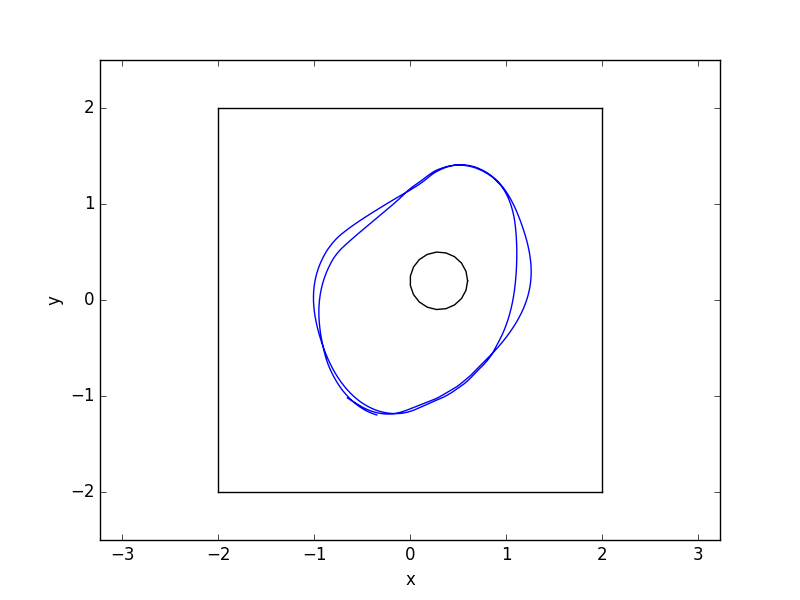
\includegraphics[width=\textwidth]{fig/2a-1.png}
			\caption{Braitenburg controller}
			\label{fig:braitenburg}
		\end{figure}

		\item The plot of the trajectory of the rule based controller is shown by figure \ref{fig:rule-based}. The basic idea is to slow down and eventually stop and reverse if the robot is about to hit an obstacle, rotating until there is a clear path. Otherwise, the robot will just go forward. There are 3 branches for different values of the front sensor. Less than 1, the speed increases linearly from -2m/s up to 1m/s, with it rotating until it can escape this branch (by finding a direction with no obstacles diredtly in front). Between 1 and 2, speed increases linearly again and the robot rotates, but slower.  Similarly, there are two branches for the front\_left and front\_right sensors for the case that there is an off centre obstacle that the front sensor doesn't detect. Similar to the braitenburg, the robot will attempt to rotate away from the obstacle depending on which sensor it is. If the robot is not close to an obstacle, it will just move forward with no rotation.
		\begin{figure}[h!]
			\centering
			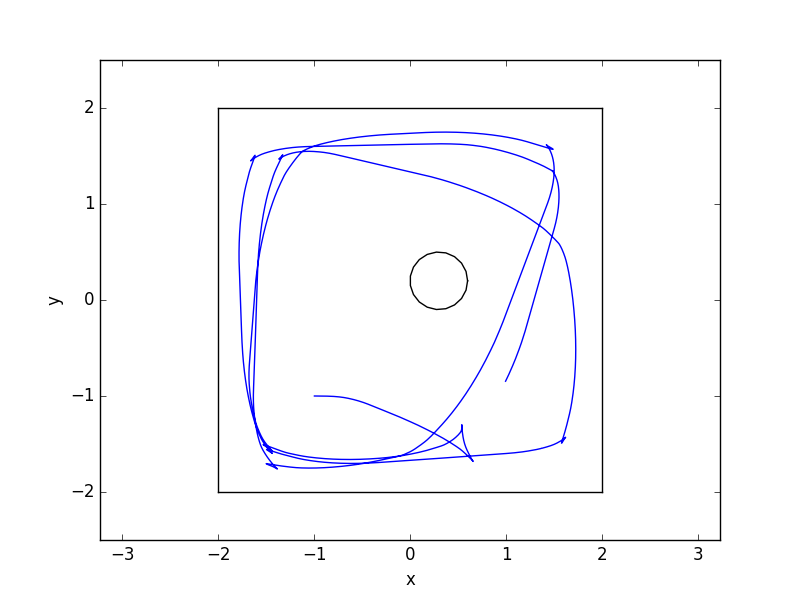
\includegraphics[width=\textwidth]{fig/2b.png}
			\caption{Rule-based controller}
			\label{fig:rule-based}
		\end{figure}

		\item The braitenburg controller is fairly robust in the face of unexpected obstacles, but there are some cases which can cause this particular controller to get stuck. For example, putting an obstacle directly in front will cause it to crash, but it will recover and move away. Putting an obstable near but not directly in front will allow the robot to steer away before hitting the obstacle. However, if an obstacle is placed in such a way to divert the robot into another obstacle (e.g. a wall), the robot sometimes gets stuck in the wall as it is unable to rotate away.
		
		The rule based controller can handle some cases of unexpected obstacles, but cannot recover easily for others. For example, putting in an obstacle when it is moving forward will cause it to slow down and maneouvre around. A similar effect occurs when putting an obstacle slightly to the side (i.e. not directly in line of sight, but would still hit). However, it is possible to trap the robot by putting down an obstacle while it is in it's 'rotation' phase as it gets close to a wall and tries to rotate away. In this case, putting an obstacle behind it will cause it to keep moving backwards into the obstace and get stuck.

		Overall, the braitenburg controller is less robust as it can recover from less types of obstacle positions.

        \item In the presence of no noise, the braitenburg controller is more robust if it is perfectly tuned, since it will never end up hitting an obstacle even in the presence of unexpected ones. As sensor measurements are guaranteed to be perfect, it can determine its position relative to obstacles \textit{exactly}, so can make sure it doesn't hit them. However, it is possible for a braitenburg controller to get stuck in a position while not hitting an obstacle. For example, if the sensor measurements are such that u and w are both set to 0 (which is possible because of negative weights), then the robot woudl not move despite not hitting any obstacles. The rule based controller will not be able to cover all the cases necessary to handle any obstacle position. However, it is likely more robust in general since it is hard to tune a braitenburg controller perfectly, and they can still get stuck.

	\end{enumerate}
\section*{1.2 Localization}
\subsection*{Exercise 3}
\begin{enumerate}[label=(\alph*)]
	\item The setup and code for my braitenburg controller is shown below:\\
	\begin{verbatim}
		def braitenberg(front, front_left, front_right, left, right):
    s = np.array([[left, front_left, front, front_right, right]])
    s = np.vectorize(lambda x: 1./x)(s)
    s = np.transpose(s)
    ws = np.array([[0.25, 0.05, 0.05, 0.05, 0.25],
                   [-0.4, -1.2, -0.4, 1.5, 0.4]])

    vs = ws.dot(s)
    u = vs[0][0] + 0.2
    w = vs[1][0] + 0.1
    return u*0.5, w*0.7

	\end{verbatim}
	\begin{figure}[h!]
		\centering
		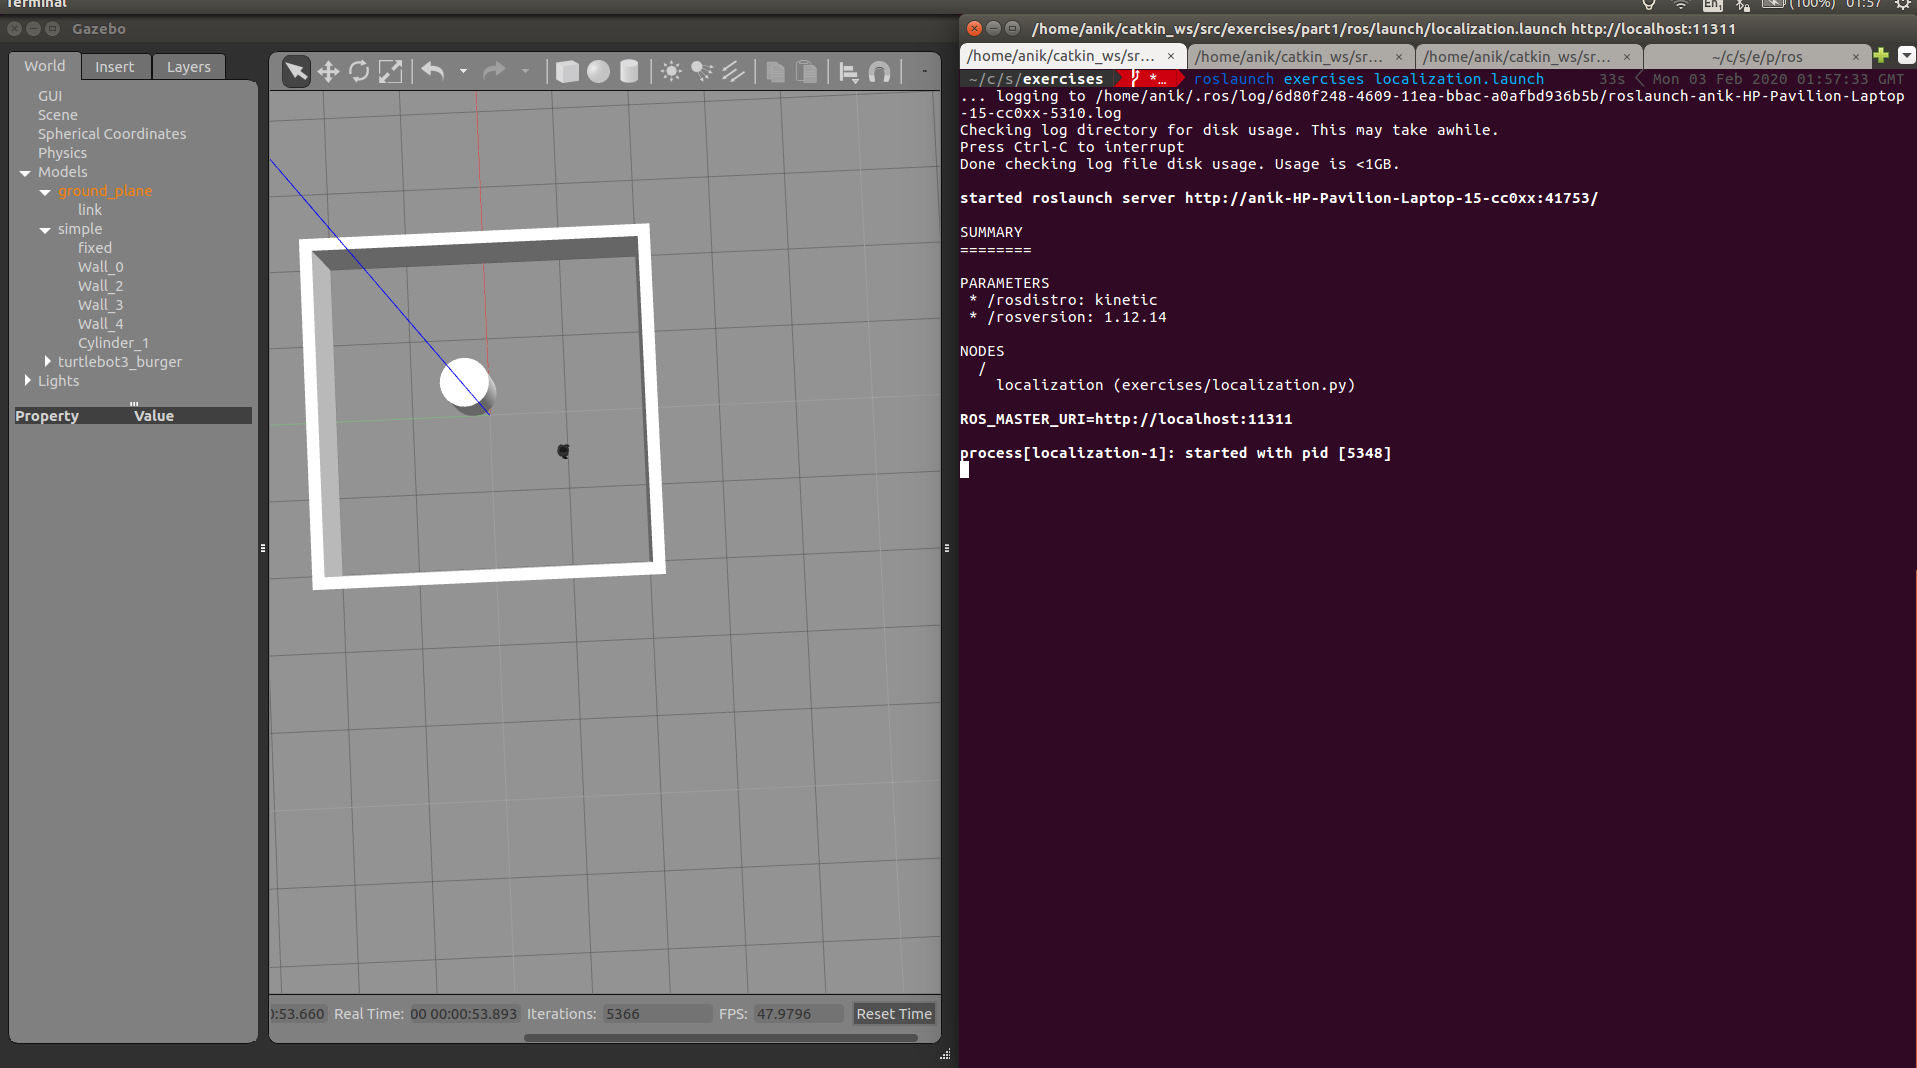
\includegraphics[width=\textwidth]{fig/3a.png}
		\caption{Gazebo setup}
		\label{fig:gazebo}
	\end{figure}

	\item My solution generates points uniformly inside the square, i.e. from -2 to 2 in both the x and y components. It also makes sure that the robot will not intersect a wall, i.e. that the centre of the robot is placedso that its radius escapes the square. It also generates a random direction (from 0 to $2\pi$) uniformly. It then checks to see whether the robot has been placed within the cylinder, and if it has, generates a new random pose since the robot cannot be inside the object. It continues until it returns a valid pose (which isnt inside the cylinder). 
	
	Setting the weight to 1 ensures that at the beginning, all these particles are equally likely.

	\item The move function takes delta\_pose, which is an offset relative to the particle. From this, I take the x and y components and add a gaussian error with a standard deviation of 10\% of the magnitude of the movement. This x and y with the noise added is added to the pose of the particle. The same is done for the yaw component.

	\begin{figure}[h!]
		\centering
		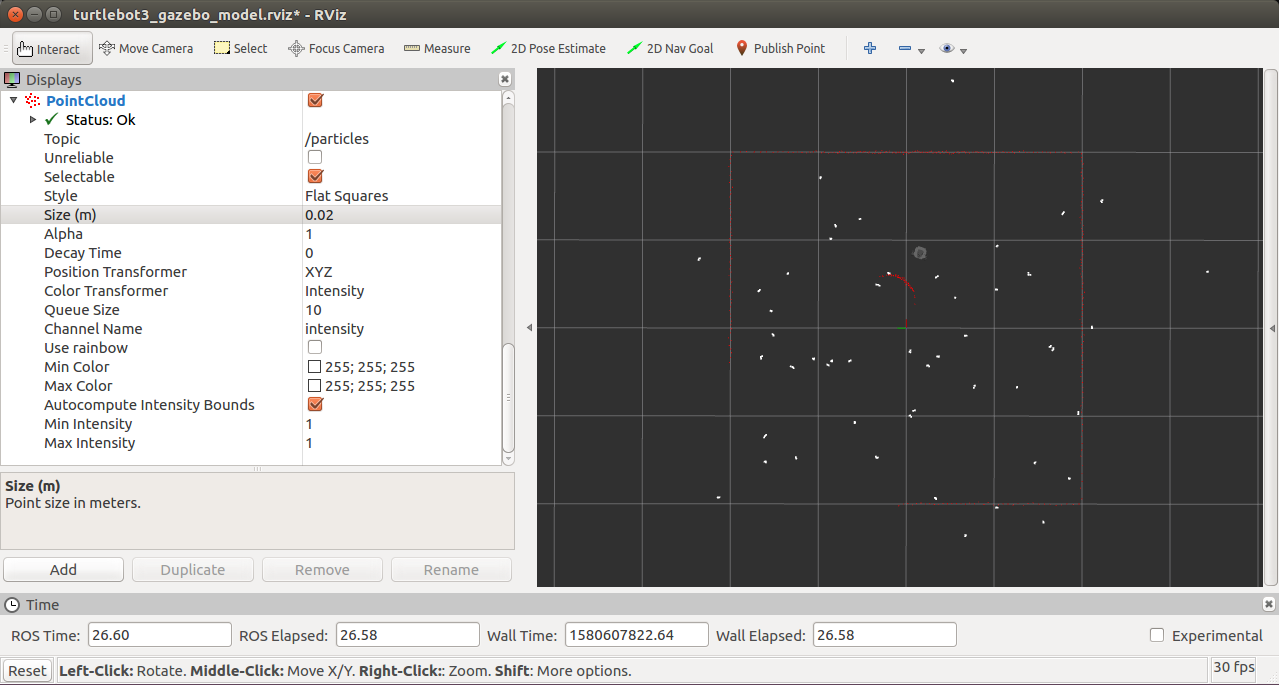
\includegraphics[width=\textwidth]{fig/3c.png}
		\caption{Rviz setup}
		\label{fig:rviz}
	\end{figure}

	\item The compute\_weight method calculated the new weight of a particle and updates it. If the particle moved outside the arena, then its weight is set to 0 so that it isn't sampled again. For the other particles, their weights are set to $ p(z|x) $, which is the probability of the measurement given the position of the particle. The measurement model is a set of normals centered around the measured value with a standard deviation of 80cm. The particles which are more likely to be in the correct postion are therefore given a higher weight, and so are much more likely to be resampled. I take an average of the probabilities of each sensor and use that as the updated weight.

	\item The localization always succeeds, but does not always converge quickly. When the particles are randomly initialised, they will not always cluster towards the position of the robot and will cluster somewhere else which is a symmetric position to the robots real position. This is because the sensor measurements from two symmetric positions will be the same, so the particles will converge to that position thinking that the robot is there since the $p(z|x)$ will be high, since the sensor reading also correspond tot aht position. This can be caused by the initial particle cloud spawning particles in unlikely positions and unluckily resampling in the wrong direction.

	\item Kidnapping still allows it to succeed, but it may take time to converge. The move function can be changed to take into account a random movement (spawn a new random particle with a low probability) to make converging to a new location faster. If this random particle is generated somehwere other than the position, the particle will die out as it will have a very low weight and not be resampled, but if it is generated near the new position, it will stay and cause more particles to converge there due to its higher weight. We can tune how likely these random particles are to ensure that the localisation can eventually recover. 

	\item Figure \ref{fig:localization} shows how quickly the particles converge.To begin with, the particles are random so the error is very high, but the resampling process reduces this error until there is only a small error remaining. There is also a plateau that can be seen on the graph before the large drop - this shows how the particles initially cluster, but converge to the wrong location. There are also some random spikes in error even by the end of the graph, which shows the random particles being generated with a low probability (they help with the kidnapping problem).
	\begin{figure}[h!]
		\centering
		\subfloat[Trajectory]{{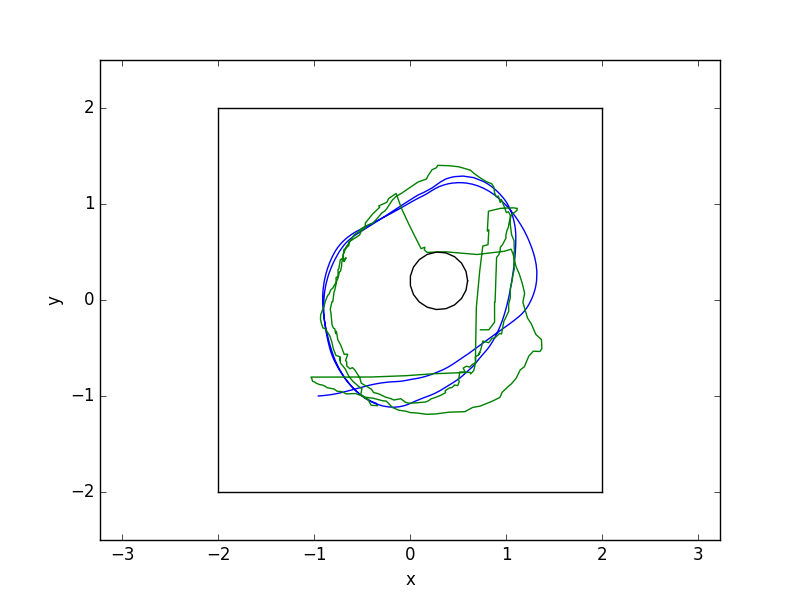
\includegraphics[width=7cm]{fig/3g-map.png}}}%
		\qquad
		\subfloat[Error]{{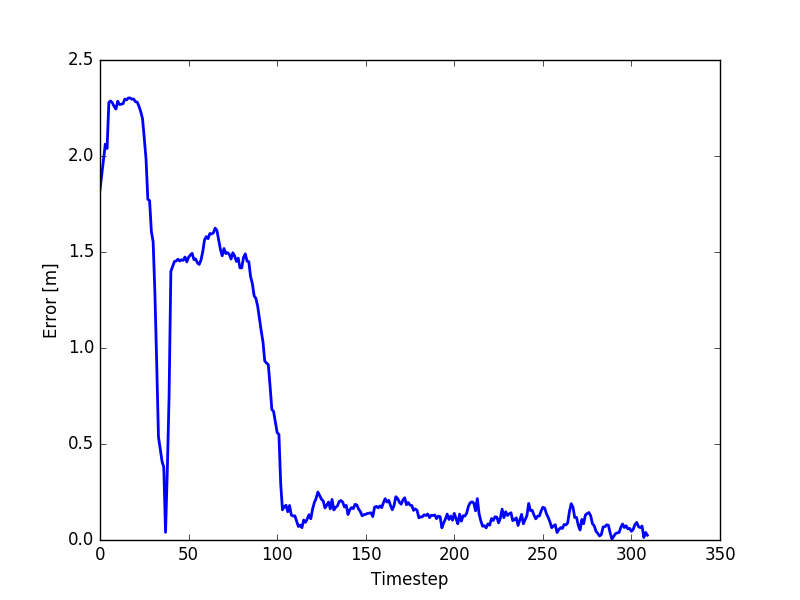
\includegraphics[width=7cm]{fig/3g-graph.png}}}%
		\caption{Localization - convergence of particles}%
		\label{fig:localization}%
	\end{figure}

	\item An extended Kalman Filter can improve the resolution of the localisation, and so can produce more accurate locations. Using gaussians directly as in the kalman filter will be more accurate since we do not rely of a 'cloud' of particles - the particles will not all end up in the same place since the cloud is randomly resampled. The Kalman filter is also more efficient since you do not do calculations for a large number of particles, you just compute probabilities for a few gaussians so you need to store and compute less. An extended Kalman Filter uses landmarks as its measurement model, so this means it must know the locations of certain landmarks on the map. It also needs to take an initial pose, whereas the particle filter does not since it can generate initial particles randomly. The Kalman filter is however less robust, since kidnapping the robot will make it quite hard for the filter to recover, since the gaussian around the location will have a low chance to change to the new position, whereas the particle filter has the ability to spawn new ranodm particles.
\end{enumerate}




\end{document}
